\documentclass[12pt, twoside]{article}
\usepackage[letterpaper, margin=1in, headsep=0.5in]{geometry}
\usepackage[english]{babel}
\usepackage[utf8]{inputenc}
\usepackage{amsmath}
\usepackage{amsfonts}
\usepackage{amssymb}
\usepackage{tikz}
%\usetikzlibrary{quotes, angles}

\usepackage{graphicx}
\usepackage{enumitem}
\usepackage{multicol}

\usepackage{fancyhdr}
\pagestyle{fancy}
\fancyhf{}
\renewcommand{\headrulewidth}{0pt} % disable the underline of the header

\fancyhead[RE]{\thepage}
\fancyhead[RO]{\thepage \\ Name: \hspace{3cm}}
\fancyhead[L]{BECA / Dr. Huson / 10th Grade Geometry\\* Unit 8 Transformations\\8 March 2019}

\begin{document}
\subsubsection*{8-4a Do Now: Applying Algebra to Geometric Situations}
  \begin{enumerate}

  \item The line $l$ has the equation $y=\frac{3}{2}x+7$. To each line below, circle whether $l$ is parallel, perpendicular, or neither.
    \begin{enumerate}
      \item parallel \quad perpendicular \quad neither \qquad $y=-\frac{2}{3}x-2$
      \vspace{0.5cm}
      \item parallel \quad perpendicular \quad neither \qquad $y=\frac{3}{2}x+9$
      \vspace{0.5cm}
      \item parallel \quad perpendicular \quad neither \qquad $2x-3y=-5$
      \vspace{1.5cm}
      \item parallel \quad perpendicular \quad neither \qquad $3x+2y=6$
      \vspace{1.7cm}
    \end{enumerate}

    \item What is the equation of a line through the point $A(-1,3)$ and parallel to the line $y=\frac{1}{2}x-5$? (hint: use the point-slope formula, $y-y_A=m (x-x_A)$) \vspace{1.5cm}

  \item Simplify each expression. (Leave it in radical form if necessary, not a decimal.)
    \begin{enumerate}
      \begin{multicols}{2}
      \item   $\sqrt{18}$ \vspace{1.5cm}
      \item   $\sqrt{\frac{1}{9}}$ \vspace{1.5cm}
      \end{multicols}
    \end{enumerate}
    \vspace{0.5cm}


  \item Write down the center and radius of each circle.
    \begin{enumerate}
      \begin{multicols}{2}
      \item   $(x+5)^2+y^2=36$ \vspace{2cm}
      \item   $(x-3)^2+(y+1)^2=72$
      \item   $(x-3)^2+(y-3)^2=5^2$ \vspace{2cm}
      \item   $(x+4)^2+(y+8)^2=9$
      \end{multicols}
    \end{enumerate}  \vspace{2cm}

\newpage

  \item $\triangle ABC$, specified below, undergoes two tranformations. First, it is rotated $90^\circ$ counterclockwise around $B$. Then it is translated $x \rightarrow x+3$, $y \rightarrow y-6$. Complete a table showing the coordinates of the translated points and plot the three triangles on the grid.\\[1cm]
   \hspace{1cm} $A(-7,3) \rightarrow$\\[1cm]
   \hspace{1cm} $B(-3,3) \rightarrow$\\[1cm]
   \hspace{1cm} $C(-4,-2) \rightarrow$

    \vspace{0.5cm}

      \begin{center} %4 quadrant regents grid w T-Chart
      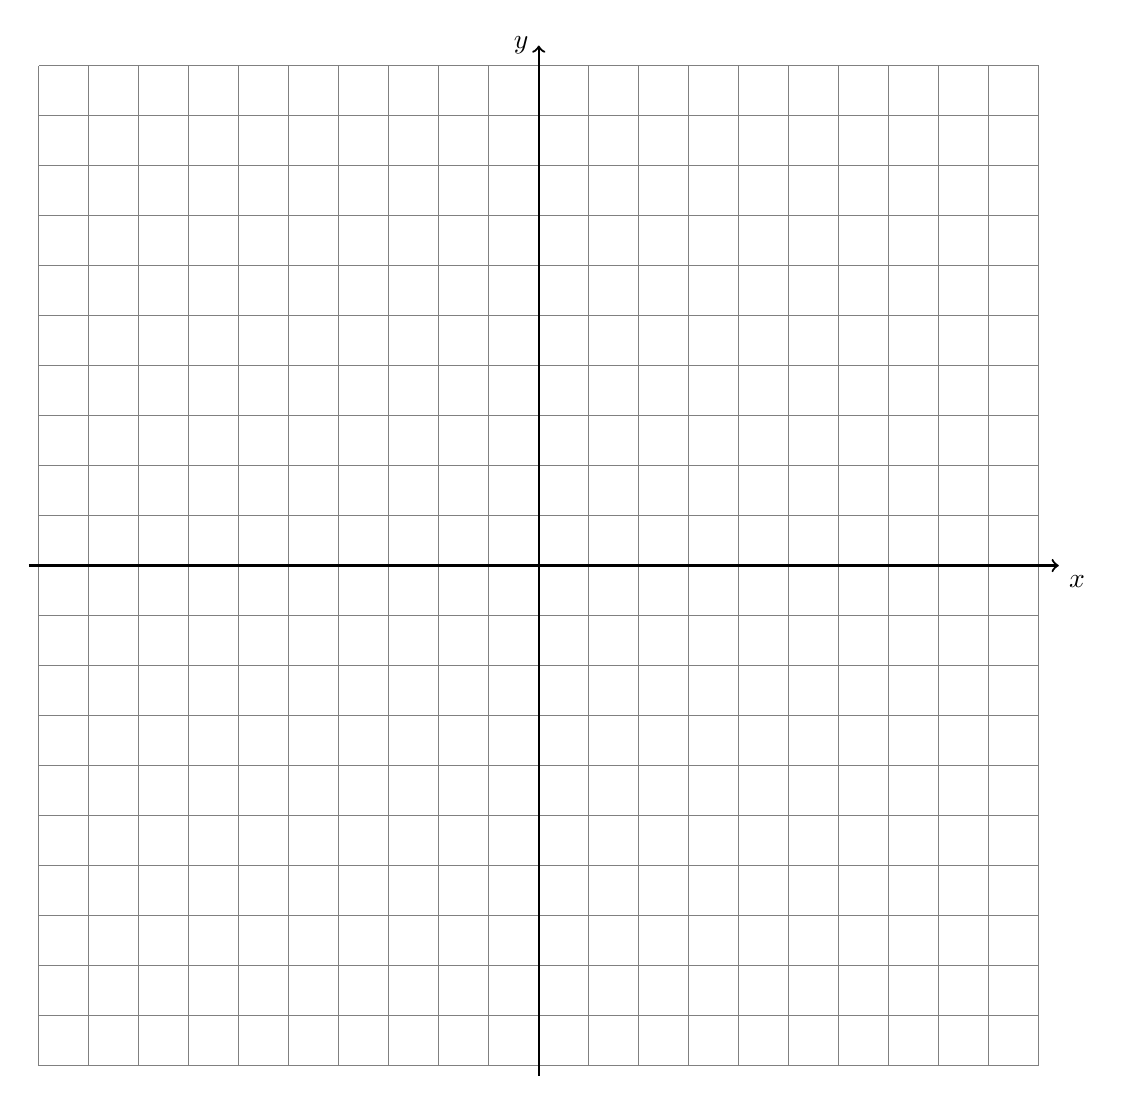
\begin{tikzpicture}[scale=.635]
        \draw [help lines] (-10,-10) grid (10,10);
        \draw [thick, ->] (-10.2,0) -- (10.4,0) node [below right] {$x$};
        \draw [thick, ->] (0,-10.2)--(0,10.4) node [left] {$y$};
      \end{tikzpicture}
      \end{center}

\end{enumerate}

\newpage

\subsubsection*{8-4a Classwork: Distance formula, line segments}
 \begin{enumerate}

  \item A translation maps $A(3,2) \rightarrow A'(5,7)$. What is the image of $B(-8,5)$ under the same translation?  \vspace{3cm}

  \item As shown below, what is the translation that maps the point $R(-3,2)$ onto the point $S(6, 5)$?
    \begin{center} %4 quadrant regents grid
      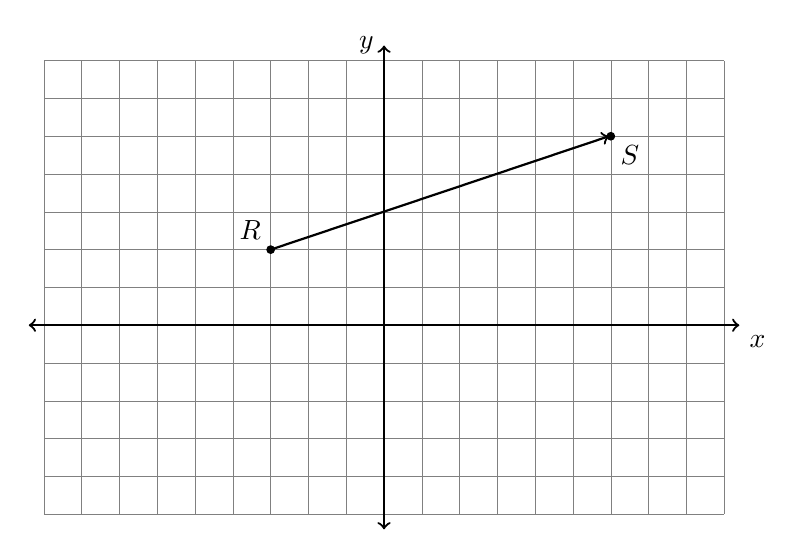
\begin{tikzpicture}[scale=.48]
        \draw [help lines] (-9,-5) grid (9,7);
        \draw [thick, <->] (-9.4,0) -- (9.4,0) node [below right] {$x$};
        \draw [thick, <->] (0,-5.4)--(0,7.4) node [left] {$y$};
        \draw [thick, ->] (-3,2)--(5.95, 5);
        \draw [fill] (-3,2) circle [radius=0.1] node[above left] {$R$};
        \draw [fill] (6, 5) circle [radius=0.1] node[below right] {$S$};
      \end{tikzpicture}
    \end{center}
    If only one third of that translation was performed, what coordinates would $R$ be mapped to? \vspace{2cm}

  \item Given $A(-2,4)$ and $B(3,-1)$, find the length of $\overline{AB}$. Leave the result in simplified radical form (not a decimal).
      \vspace{4cm}

\newpage

  In the following two problems, solve for the value of $x$.
  \begin{multicols}{2}
  \item   $\frac{1}{5}(2x+3)=1$ \vspace{6cm}
  \item   $\frac{1}{3}(21-3x)=5$ \vspace{6cm}
  \end{multicols}

\vspace{3cm}

  \item Given $f(x)=\frac{1}{4} x+4$. Solve for $x$ such that for $f(x)=6$. \vspace{3.5cm}
  \item Given $g(x)=3x^2-7x+5$. Simplify $g(0)$. \vspace{3cm}
  \item Given $f(x)=5x-22$. Solve for $x$ such that for $f(x)=3$. \vspace{3.5cm}
  \item Given $h(x)=x^2+6x+5$. Solve $h(x)=0$. \vspace{3cm}


  \end{enumerate}

  \end{document}
